%------------------------------------------------------------------------------
% Beginning of journal.tex
%------------------------------------------------------------------------------
%
% AMS-LaTeX version 2 sample file for journals, based on amsart.cls.
%
%        ***     DO NOT USE THIS FILE AS A STARTER.      ***
%        ***  USE THE JOURNAL-SPECIFIC *.TEMPLATE FILE.  ***
%
% Replace amsart by the documentclass for the target journal, e.g., tran-l.
%
\documentclass{amsart}
%     If your article includes graphics, uncomment this command.
\usepackage{amsthm,graphicx,amssymb,textcomp,cancel,bbm,enumerate,svg,graphicx,caption,listings}
\usepackage{listings-golang}

\setcounter{section}{-1}

\newtheorem{theorem}{Theorem}%[section]
\newtheorem{lemma}[theorem]{Lemma}

\theoremstyle{definition}
\newtheorem{definition}{Definition}
\newtheorem{example}[theorem]{Example}
\newtheorem{xca}[theorem]{Exercise}

\theoremstyle{remark}
\newtheorem{remark}[theorem]{Remark}
\newtheorem*{remark*}{Remark}

\theoremstyle{definition}
\newtheorem{notation}[theorem]{Notation}

\numberwithin{equation}{section}
%\setcounter{section}{-1}
%%
\mathchardef\ordinarycolon\mathcode`\:
\mathcode`\:=\string"8000
\begingroup \catcode`\:=\active
  \gdef:{\mathrel{\mathop\ordinarycolon}}
\endgroup


\newcommand\nsleq{\mathrel{\ooalign{$\leqslant$\cr\hidewidth$|$\hidewidth\cr}}}
\newcommand{\sleq}{\leqslant}
\newcommand{\No}{\mathbb{N}\bf{o}}
\newcommand{\abs}[1]{\lvert#1\rvert}

%    Blank box placeholder for figures (to avoid requiring any
%    particular graphics capabilities for printing this document).
\newcommand{\blankbox}[2]{%
  \parbox{\columnwidth}{\centering
%    Set fboxsep to 0 so that the actual size of the box will match the
%    given measurements more closely.
    \setlength{\fboxsep}{0pt}%
    \fbox{\raisebox{0pt}[#2]{\hspace{#1}}}%
  }%
}

\begin{document}
\title{Numerical Analysis Programming Project \\ Dr. Songming Hou}
\author{John Emory}
\address{Program of Mathematics and Statistics, Louisiana Tech University}
\email{jfe004@latech.edu}
\date{\today}
\maketitle

\section{Introduction}
Tom the Cat is chasing Jerry the Mouse, with an initial gap between them of $100$m. Tom and Jerry's velocities
are given as $v_c = 4 - at$ ms$^{-1}$ and $v_m = v_{max}-ks = 3 - 0.02s$ ms$^{-1}$, respectively,
with $0<a$.
The velocity of the change in the gap between Tom and Jerry, $s$, is given by
$\frac{ds}{dt} = v_m - v_c = -1 -0.02s + at$ ms$^{-1}$.

\section{Problem}
Find the true solution for when Tom will catch Jerry by plotting the gap distance.
\\
\\
First, we need to solve $\frac{ds}{dt}$. Noting that our equation is a linear first-order ODE, we
need to put it into standard form:
\[\frac{ds}{dt} + 0.02s = at -1\]
Next, we find the integration factor. Observing that in the second additive term on the left hand side
we are multiplying by $t^0$, we see the integration factor is $e^{0.02t}$. This gives us the form:
\[\frac{d}{dt}s\cdot e^{0.02t} = ( at-1 )\cdot e^{0.02t}\]
Taking the antiderivative of both sides gives:
\[\int\frac{d}{dt}s\cdot e^{0.02t} dt = a\cdot \int t \cdot e^{0.02t} dt - \int e^{0.02t} dt\]
\[s\cdot e^{0.02t} = 50at\cdot e^{0.02t} = 2500a\cdot e^{0.02t} - 50e^{0.02t} +c\]
Then, canceling $e^{0.02t}$ gives:
\[s = 50a(t-50)-50+c \cdot e^{-0.02t}\]
Solving for $c$ at our initial value of $s(0)=100$ m will yield an equation we can use software to plot. Since $t=0$, we have:
\[100=-2500a-50+c \cdot e^{-0.02t}\]
\[c = 2500a + 150\]
So, our final equaiton we want to plot is:
\[s(a,t) = 50a(t-50+50\cdot e^{-0.02t})+150\cdot e^{-0.02t} -50\]

\begin{figure}
  \centering
  \begin{center}
    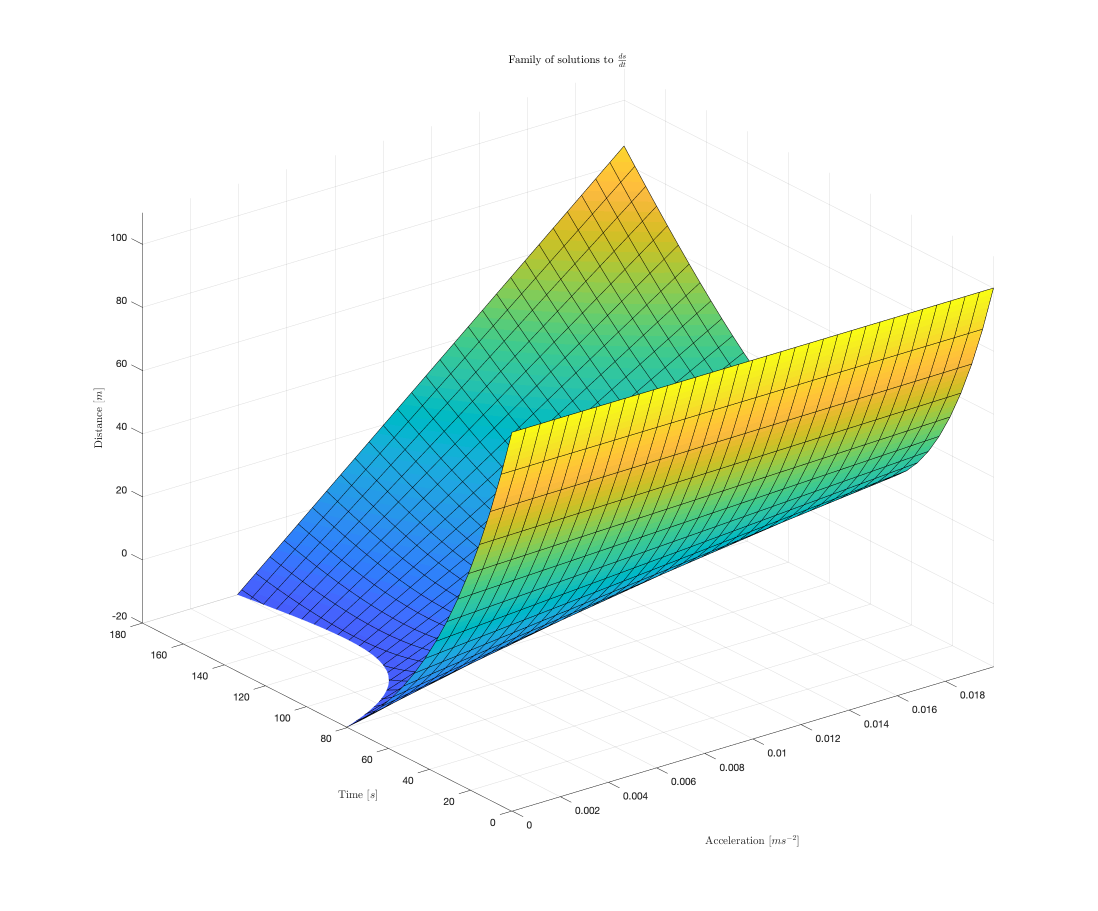
\includegraphics[scale=0.13]{3dPlot-NumericalFinal.jpg}
    \caption{Plot of solutions to $\frac{ds}{dt}$}
  \end{center}
\end{figure}

The exact solutions to when Tom catches Jerry are the points on the surface in Figure 1 that intersect with
the plane at $s=0$ with minimal $t$ value. This can be seen in the figure as the curve traced
by the surface where it intersects the bottom of the plot. The plot indicates that at $a=0.01$ m$s^{-1}$, Tom
will catch Jerry at roughly 82 seconds.
\section{Problem}
For $a = 0.01$ ms$^{-2}$, use the fourth-order Runge-Kutta method to compute when Tom will catch Jerry.
Use an appropriate step size to ensure an accurate result.
\\
\\
The source code for both Runge-Kutta and Adams-Bashforth is attached as Appendix 1, and at
https://github.com/jfemory/numericalAnalysisFinal. From Table \ref{RKout}, the condensed
output of the fourth-order Runge-Kutta calculations, we see that Tom catches Jerry between
81.5 and 82 seconds, when the sign of the distance changes to negative.

\begin{table}[h]
  \caption{Runge-Kutta Output} %title of the table
  \centering % centering table
  \begin{tabular}{c rrrrrrr} % creating eight columns
  \hline\hline %inserting double-line
  Time (s) & 80.0 & 80.5 & 81.0& 81.5& 82.0& 82.5& 83\\ % Entering row contents
  Distance (m) & 0.3319 & 0.2303 & 0.1323& 0.0377& -0.0535& -0.1413& -0.2257\\
  \hline % inserts single-line
  \end{tabular}
  \label{RKout}
  \end{table}

\section{Problem}
Use the Adams-Bashforth forth-order predictor-corrector to compute when Tom will catch Jerry using the
results form Runge-Kutta, above, for the initial values of Adams-Bashforth.
\\
\\
Similar to the previous question using the Runge-Kutta technique, relevant values
near the sign change for the Adams-Bashforth are given in Table \ref{ABout}.
\begin{table}[h]
  \caption{Adams-Bashforth Output} %title of the table
  \centering % centering table
  \begin{tabular}{c rrrrrrr} % creating eight columns
  \hline\hline %inserting double-line
  Time (s) & 80.0 & 80.5 & 81.0& 81.5& 82.0& 82.5& 83\\ % Entering row contents
  Distance (m) & 0.3319 & 0.2303 & 0.1323& 0.0377& -0.0535& -0.1413& -0.2257\\
  \hline % inserts single-line
  \end{tabular}
  \label{ABout}
  \end{table}

  It can be seen that the Tables 1 and 2 are in agreement up to four decimal places.
  The results between the two methods do in fact differ at higher precision. Please see
  Apendix 2 for a complete comparison at precision. The initial four values from Runge-Kutta
  were used as input for the Adams-Bashforth method.

\section{Problem}
Suppose Tom's acceleration is unknown. If Tom does not catch Jerry in $120$s, is it possible that Tom
will catch Jerry?
\\
\\
No. It is not possible. Figure 2 indicates the accelerations and times where the gap is less
than zero. The border of the blue area indicates where the sign of the gap changes. So, we can see can see
that any constant acceleration path (horizontal lines) that does
not reduce the gap to 0m by 120s has no solutions to the
right of 120s. In other words, any constant acceleration path
that has a zero to the right of 120s also has a zero to the left of 120s. Therefore, no,
if tom has not caught Jerry by 120s, Tom will never catch Jerry.

\begin{figure}
  \centering
  \begin{center}
    \includegraphics[scale=0.12]{2dPlot-NumericalFinal.jpg}
    \caption{Time vs Acceleration Zeros}
  \end{center}
\end{figure}

\appendix
\section{Runge-Kutta and Adams-Bashforth Source Code (Golang)}
\lstinputlisting[language=Golang]{NumericalMethods.go}
\newpage
\section{3d Plot Source Code (Matlab)}
\lstinputlisting[language=Matlab]{PlotDiffEQ.m}
\newpage
\section{2d Plot Source Code (Matlab)}
\lstinputlisting[language=Matlab]{PlotDiffEQ2d.m}
\newpage
\section{Complete Tables}
\end{document}